% 建议使用 XeLaTeX 或 LuaLaTeX 编译(中文与公式支持更佳)
\documentclass[UTF8,zihao=-4]{ctexart}

\usepackage[a4paper,margin=2.5cm]{geometry}
\usepackage{amsmath, amssymb, amsthm}
\usepackage{bm}
\usepackage{hyperref}
\usepackage{graphicx}
\usepackage{caption}
\usepackage{listings}
\usepackage{xcolor}
\usepackage{float}
\usepackage{placeins}
\graphicspath{{figures/}}

\lstdefinestyle{code}{
  basicstyle=\ttfamily\small,
  numbers=left,
  numberstyle=\tiny,
  numbersep=8pt,
  keywordstyle=\color{blue},
  commentstyle=\color{teal!70!black},
  stringstyle=\color{orange!70!black},
  showstringspaces=false,
  breaklines=true,
  frame=single,
  framerule=0.3pt,
  rulecolor=\color{black!15}
}
\lstset{style=code}

\title{独立成分分析:原理、公式、应用与实战}
\author{}
\date{\today}

\begin{document}
\maketitle

\section{引言}
独立成分分析(Independent Component Analysis, ICA)通过高阶统计量将混合的观测信号拆解为互相独立的潜在源。与只消除二阶相关性的主成分分析(PCA)不同,ICA 借助非高斯性最强的投影方向实现盲源分离,广泛应用于多声道音频、功能性脑影像和高光谱成像等场景。由于 ICA 保留了线性生成模型,被恢复的成分还可回混获得原始信号,从而具备良好的可解释性。

\section{原理与公式}
\subsection{线性混合模型}
设观测向量 \(\mathbf{x} \in \mathbb{R}^m\) 由 \(n\) 个独立源 \(\mathbf{s}\) 经可逆混合矩阵 \(\mathbf{A} \in \mathbb{R}^{m \times n}\) 线性组合而来:
\begin{equation}
\mathbf{x} = \mathbf{A}\mathbf{s}, \qquad \mathbb{E}[\mathbf{s}] = \mathbf{0}, \qquad \operatorname{Cov}(\mathbf{s}) = \mathbf{I}.
\end{equation}
ICA 旨在估计解混矩阵 \(\mathbf{W}\),使 \(\hat{\mathbf{s}} = \mathbf{W}\mathbf{x}\) 近似原始源信号。由于交换或取反某个源并相应调整 \(\mathbf{W}\) 仍可保持观测不变,解具有排列与符号的不确定性。

\subsection{非高斯性与对比函数}
核心思想是:独立非高斯变量的任意线性组合往往比原始变量更趋近高斯分布(中央极限定理)。因此可最大化投影 \(y = \mathbf{w}^\top \mathbf{z}\) 的非高斯程度,其中 \(\mathbf{z}\) 表示白化后的数据。常用的对比函数包括峰度与近似负熵:
\begin{align}
\text{Kurt}(y) &= \mathbb{E}[y^4] - 3,\\
J(y) &\approx \left(\mathbb{E}[G(y)] - \mathbb{E}[G(v)]\right)^2,
\end{align}
其中 \(v\) 为标准高斯变量,\(G\) 为非二次函数,如 \(G(y)=\log \cosh(y)\)。FastICA 的迭代更新为
\begin{equation}
\mathbf{w}_{\text{new}} = \mathbb{E}[\mathbf{z}g(\mathbf{w}^\top\mathbf{z})] - \mathbb{E}[g'(\mathbf{w}^\top\mathbf{z})] \mathbf{w}, \qquad g = G'.
\end{equation}
每次迭代后需对向量与已有成分正交化,从而保证结果彼此独立。

\subsection{白化、似然与收敛}
预先对白化数据(\(\mathbf{z}=\mathbf{V}^{-1/2}(\mathbf{x}-\bar{\mathbf{x}})\))能消除二阶相关,将问题化简为寻找正交矩阵。亦可从最大似然角度出发,最小化独立成分间的互信息:
\begin{equation}
\min_{\mathbf{W}} I(\hat{s}_1, \dots, \hat{s}_n) = \sum_{i=1}^n H(\hat{s}_i) - H(\hat{\mathbf{s}}),
\end{equation}
其中 \(H\) 为微分熵。实际实现通常通过监控相邻迭代中 \(\mathbf{w}\) 的夹角或对数似然的变化来判定收敛,并在必要时加入小的正则项以提升数值稳定性。

\section{应用与技巧}
\begin{itemize}
  \item \textbf{盲源分离}:在鸡尾酒会问题中分离多路语音,或在 fMRI/EEG 中提取功能网络与噪声源。
  \item \textbf{稀疏特征构造}:在自然图像上训练 ICA,可得到局部化、类似边缘的滤波器,用于识别或压缩。
  \item \textbf{金融与工业监测}:独立成分能够揭示潜在风险因子或设备故障模式,补充传统相关性分析。
  \item \textbf{实用建议}:务必居中并白化数据,尝试不同的对比函数,多次随机初始化,并借助相关系数或互信息诊断结果的独立性。
\end{itemize}

\section{Python 实战}
脚本 \texttt{gen\_ica\_figures.py} 构造正弦、方波与拉普拉斯噪声三类独立源,经随机矩阵混合后使用 FastICA 分离,输出源/混合/恢复信号对比以及混合矩阵热力图。核心流程如下所示。
\begin{lstlisting}[language=Python,caption={脚本 gen_ica_figures.py 片段}]
from sklearn.decomposition import FastICA

ica = FastICA(
    n_components=3,
    whiten=True,
    max_iter=1000,
    tol=1e-4,
    random_state=0,
)
sources_hat = ica.fit_transform(mixed_signals)

mixing = ica.mixing_
unmixing = ica.components_
correlations = np.corrcoef(true_sources, sources_hat, rowvar=True)
\end{lstlisting}
通过检查 `correlations` 中的最大绝对值,可验证恢复成分与原始源是否一一对应(忽略符号与排列)。

\section{实验结果}
\begin{figure}[H]
  \centering
  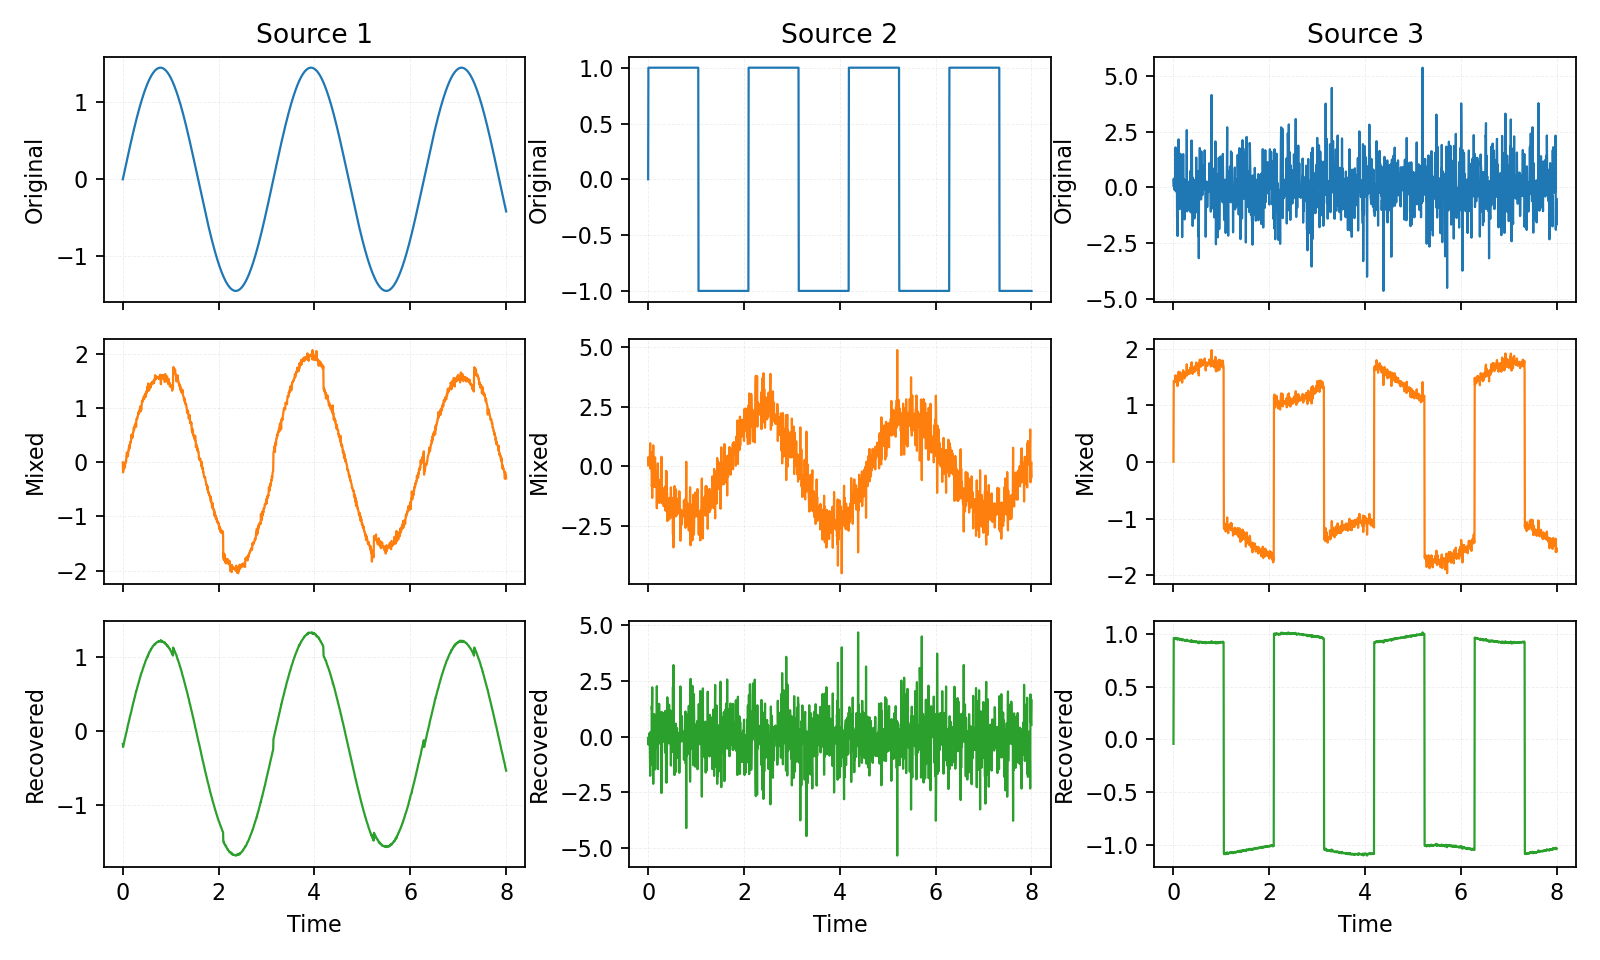
\includegraphics[width=0.85\linewidth]{ica_sources_vs_recovered.png}
  \caption{三路信号的原始源、混合观测与 ICA 恢复结果对比}
  \label{fig:ica_sources_vs_recovered_cn}
\end{figure}

\begin{figure}[H]
  \centering
  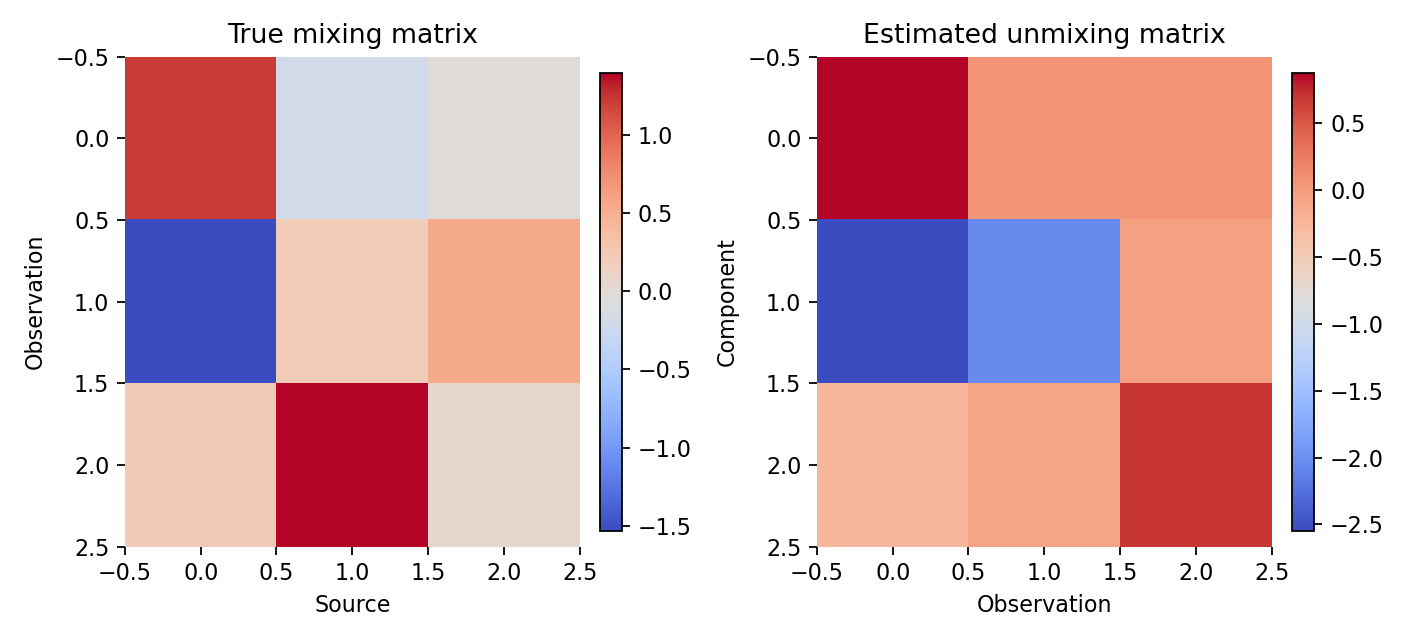
\includegraphics[width=0.75\linewidth]{ica_mixing_matrices.png}
  \caption{真实混合矩阵(左)与估计解混矩阵(右)的热力图,非对角元素提示残余混合}
  \label{fig:ica_mixing_matrices_cn}
\end{figure}

\FloatBarrier
\section{总结}
ICA 通过最大化非高斯性在去相关基础上进一步恢复独立潜在因子。只要完成白化、选用合适的对比函数并对结果进行诊断,就能在多信号场景中实现可靠的盲源分离。合成案例示范了如何借助时间序列与矩阵可视化评估分离效果。

\end{document}
